\section{A simple example: classify handwritten digits with a multi-layer
  perceptron}

\begin{frame}
  \frametitle{The MNIST dataset}
  \begin{columns}
    \begin{column}{0.5\textwidth}
      \begin{itemize}
      \item Classic dataset
        \begin{itemize}
        \item Lots of methods have been tested with it
        \end{itemize}
      \item All images have the same size and aspect ratio (non-trivial
        pre-processing)
      \item The label is known: $\trainingSet = \setpredicate{\couple{\example_{i}}{\knownLabel_{i}}}{i=1..\nTrainingSamples}$
      \item The task is to recognize the digit on the image \ie{} we are looking
        for a function: $\decisionFunc: \, \setR^{\dimExample} \mapsto \intinterval{0}{9}$
      \end{itemize}
    \end{column}
    \begin{column}{0.5\textwidth}
      \begin{tikzpicture}[>=stealth]
        \node[anchor=south west,inner sep=0] (image) at (0,0) {
          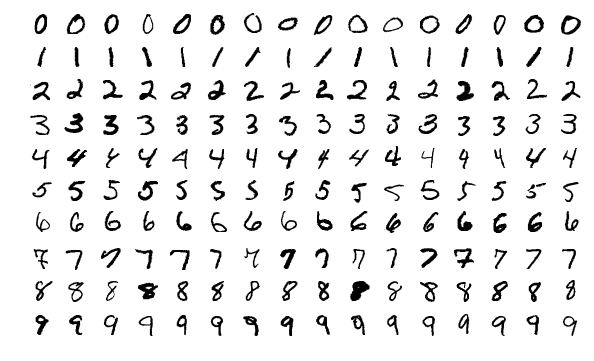
\includegraphics[width=\columnwidth]{img/MnistExamples.png}
        };
        \onslide<2->{
        \begin{scope}[x={(image.south east)},y={(image.north west)}]
          \draw[red,ultra thick] (0.22,0.15) rectangle (0.28,0.25);
        \end{scope}
        }
      \end{tikzpicture}
      \url{http://yann.lecun.com/exdb/mnist/index.html}
    \end{column}
  \end{columns}
\end{frame}

\begin{frame}
  \frametitle{Multi-layer perceptron: Introduction}

  \begin{itemize}
  \item 1957 but many improvements since
  \item Very loose biological inspiration
  \end{itemize}
\end{frame}

\begin{frame}
  \frametitle{Multi-layer perceptron: computation}
  \begin{textblock}{100}(5,10)
    \begin{tikzpicture}[>=stealth]
      % Inspired by https://tex.stackexchange.com/a/153974
      % We display a MLP with 2 hidden layers for OCR
      % The input image and the output layer are always displayed
      % The layers (input and the 2 hidden) and their connections appear after
      % Description of layers are on the graph

      % Parameters
      \def\xInputImage{0}
      \def\nameInputImage{input-name}
      \def\xInput{2.2}
      \def\nameInput{input}
      \def\xHiddenI{4.4}
      \def\nameHiddenI{hidden1}
      \def\xHiddenII{6.6}
      \def\nameHiddenII{hidden2}
      \def\xOutput{8.8}
      \def\nameOutput{output}
      \def\xProba{9.2}
      \def\nameProba{proba}
      \def\missing{missing}

      % Input image and grid
      % This part is inspired by https://tex.stackexchange.com/a/128648
      % and a lot of trial and error for the grid (including a bit of ChatGPT)
      % Apparently, the idea is to fix the size of the image and then the grid
      % flows
      % I use 56px (twice the real size) so that it looks OK and computations are easy.
      \node[anchor=center,inner sep=0pt,draw=black] (\nameInputImage) at (\xInputImage,0) {
        
\includegraphics[width=56px,height=56px]{img/Mnist_8.png}
      };
      \begin{scope}
        \clip (\nameInputImage.south west) rectangle (\nameInputImage.north east);
        \draw[step=2px,gray,very thin] (\nameInputImage.south west) grid (56px, 56px);
      \end{scope}

      \onslide<2->{
      % Input layer
      \node [align=center, above] at (\xInput,2.2) {%Input \\ layer \\
          {\tiny $28\times28=784$ units}};
      \foreach \m/\l [count=\y] in {1,2,3,missing,784}
      \node [every neuron/.try, neuron \m/.try] (\nameInput-\m) at (\xInput,3.0-\y) {};

      % Connections from input image to input layer
      % No loop here cause we need to shift the positions
      % It uses the scale introduced above
      \draw [->] (\nameInputImage)++(-27px,27px) -- (\nameInput-1);
      \draw [->] (\nameInputImage)++(-25px,27px) -- (\nameInput-2);
      \draw [->] (\nameInputImage)++(-23px,27px) -- (\nameInput-3);
      \draw [->] (\nameInputImage)++(27px,-27px) -- (\nameInput-784);

      % Description of the output
      \node[anchor=north west] at (\xInput-1, -2.2) {$\output^{1}_{k} = \matrixLinElem{\matrix{I}}{k}$} ;
      }

      % First hidden layer
      % Connections are displayed in 2 different slides (see below)
      \onslide<3->{
      \node [align=center, above] at (\xHiddenI,2.2) {%Hidden \\ layer \\
          {\tiny 200 $\ReLUFunc$ units}};
      \foreach \m [count=\y] in {1,2,missing,3}
      \node [every neuron/.try, neuron \m/.try ] (\nameHiddenI-\m) at (\xHiddenI,2.5-\y) {};
      }

      % Connections from input layer to first neuron with weights
      % and explanation of the output
      \onslide<3>{
      \foreach \p in {1,2,3,784}
      \foreach \k in {1}
      \draw[->] (\nameInput-\p) -- node {${\color{red} \weight^{2}_{\k,\p}}$} (\nameHiddenI-\k);

      % Description of the output
      \node[text width=5,anchor=north west] at (\xHiddenI-1, -2.2) {{\footnotesize
          \begin{align*}
            \begin{aligned}
              & s^{2}_{k}      & = & \sum_{p=1}^{N_{1}} {\color{red} \weight^{2}_{k,p}} \output^{1}_{p} \\
              & \output^{2}_{k} & = & \ \apply{\activFunc}{s^{2}_{k}} \\
              &                     & = & \apply{\ReLUFuncExt}{0, s^{2}_{k}}
            \end{aligned}
          \end{align*}
        }};
      }

      % Other connections from input layer to first hidden layer
      % and matrix form
      \onslide<4->{
      \foreach \i in {1,2,3,784}
      \foreach \j in {1,...,3}
      \draw[->] (\nameInput-\i) -- (\nameHiddenI-\j);
      \node[text width=3] at (\xHiddenI-1, -2.4) {{
          \begin{equation*}
            %\begin{aligned}
            \vector{\output^{2}} = \apply{\activFunc}{{\color{red}\weightMatrix^{2}}\vector{\output^{1}}}
            %\end{aligned}
          \end{equation*}
        }};
      }

      % Second hidden layer
      \onslide<5->{
      \node [align=center, above] at (\xHiddenII,2.2) {% Hidden \\ layer \\
          {\tiny 150 $\ReLUFunc$ units}};
      \foreach \m [count=\y] in {1,2,missing,3}
      \node [every neuron/.try, neuron \m/.try ] (\nameHiddenII-\m) at (\xHiddenII,2.2-0.9*\y) {};

      % Connections to first hidden layer to second hidden layer
      \foreach \i in {1,2,3}
      \foreach \j in {1,2,3}
      \draw [->] (\nameHiddenI-\i) -- (\nameHiddenII-\j);

      \node[text width=3,anchor=north west] at (\xHiddenII-1, -2.2) {{
          \begin{equation*}
            %\begin{aligned}
            \vector{\output^{3}} = \apply{\activFunc}{{\color{red}\weightMatrix^{3}}\vector{\output^{2}}}
            %\end{aligned}
          \end{equation*}
        }};
      }

      % Output layer
      \node [align=center, above] at (\xOutput,2.2) {% Output \\ layer \\
        {\tiny 10 $\softMaxFunc$ units}};
      \foreach \m [count=\y] in {0,1,missing,9}
      \node [every neuron/.try, neuron \m/.try ] (\nameOutput-\m) at (\xOutput,1.8-0.7*\y) {};

      \onslide<6->{
      % Connection from second hidden layer to output layer
      \foreach \i in {1,2,3}
      \foreach \j in {0,1,9}
      \draw [->] (\nameHiddenII-\i) -- (\nameOutput-\j);

      % Description of output
      \node[text width=3,anchor=north west] at (\xOutput-1, -2.2) {{\footnotesize
          \begin{align*}
            \begin{aligned}
              & s^{\layer+1}_{k}      & = & \sum_{p=1}^{N_{\layer}} {\color{red} \weight^{\layer}_{k,p}} \output^{\layer}_{p} \\
              & \output^{n}_{k} & = & \frac{\apply{\exp}{s^{n}_{k}}}{\sum_{j=1}^{10} \apply{\exp}{s^{n}_{j}}}
            \end{aligned}
          \end{align*}
        }};
      }

      % Output probabilities
      \foreach \m [count=\y] in {0,1,missing,9}
      \node (\nameProba-\m) at (\xProba,1.8-0.7*\y) {\ifx\m\missing\else {\tiny $\prob{\m}$}\fi};
    \end{tikzpicture}

  \end{textblock}

\end{frame}


